\documentclass{beamer}
\usetheme{Boadilla}

% \documentclass[landscape]{infslides}
% \usepackage{graphicx}
% \usepackage{multicol}
% \usepackage[export]{adjustbox}

\graphicspath{{./images/}}

\title{My Presentation}
\subtitle{Using Beamer}
\author{Joe Bloggs}
\institute{University of ShareLaTeX}
\date{\today}

\begin{document}

\begin{frame}
\titlepage
\end{frame}

\begin{frame}
\frametitle{Outline}
\tableofcontents
\end{frame}

% \title[IoTSSC Project]{IoTSSC Project\\Indoor Localisation}
% \author[Lorenzo Martinico and Piotr Jander]{Lorenzo Martinico \and Piotr Jander}
% \date{\today}

% \maketitle
% %\tableofcontents
% \begin{slide}{Tracking device}
%     Our chosen localisation device is a Nordic nRF51-DK, running ARM Mbed OS 5
%     \begin{figure}
%         \centering
%         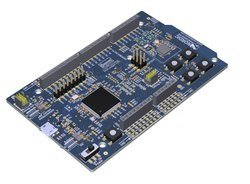
\includegraphics{nRF51-DK.jpg}
%     \end{figure}
%     Due to limited processing power, the firmware running on the board is limitied to scanning for Bluetooth Beacons and updating a BLE Characteristic with their RSSI strength
% \end{slide}
% \begin{slide}{Android App}
%     \begin{multicols}{2}
%         The app acts as a Bluetooth gateway, connecting to the board to read from its LocationService, and forward a timestamped RSSI, BeaconID pair to the server.\\
%         Additionally, we display a map of the 5th floor, and a location marker, which can be manually modified based on the board's position to collect training data.
%         \begin{figure}
%             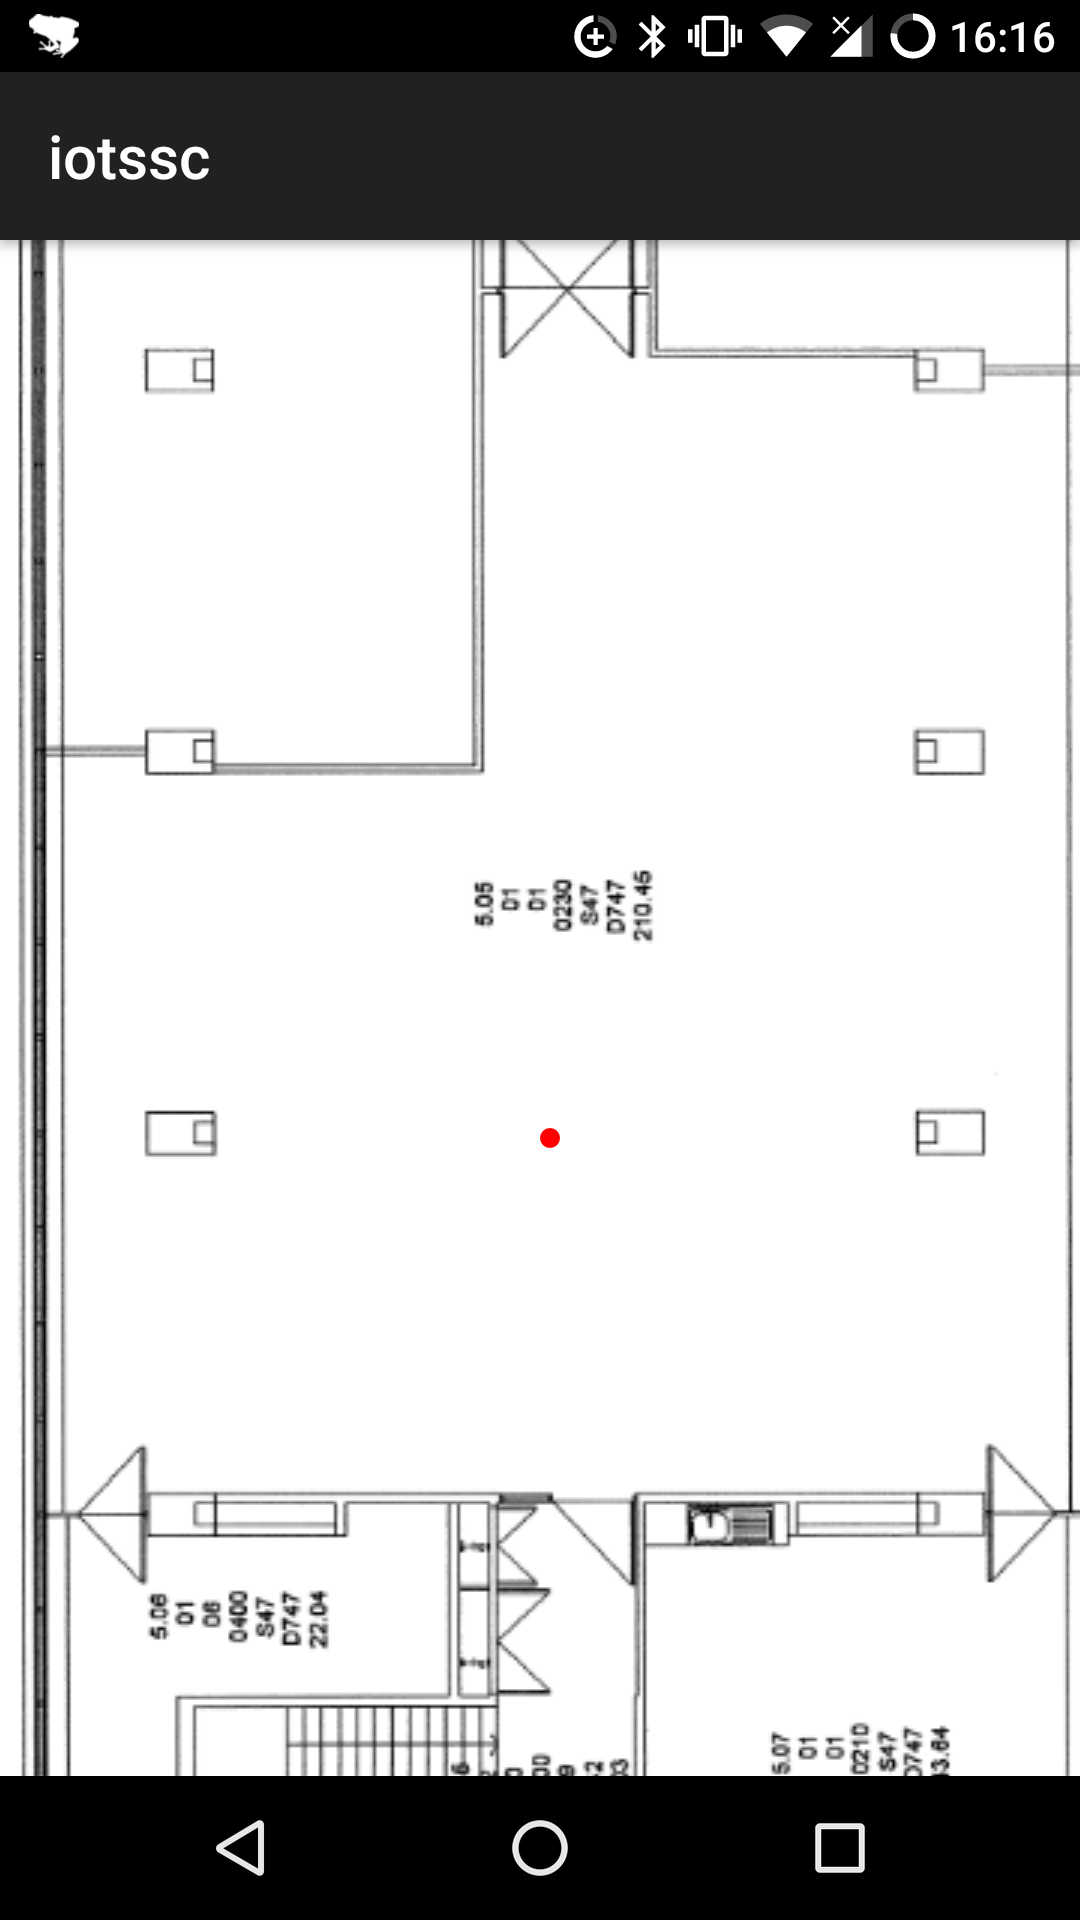
\includegraphics[scale=0.2,right]{Screenshot.png}
%         \end{figure}
%     \end{multicols}
% \end{slide}
% \begin{slide}{Server}
% The server is a simple Flask app hosted on a Google Cloud Virtual Machine. It receives POST requests from the Gateway, and saves the data in a file.

% To ensure all data is transimitted securely, the server runs over HTTPS, using a self signed certificate manually provisioned to the app (its only client).
% \end{slide}

\begin{frame}
\frametitle{Collected data}
\begin{columns}
\column{0.5\textwidth}
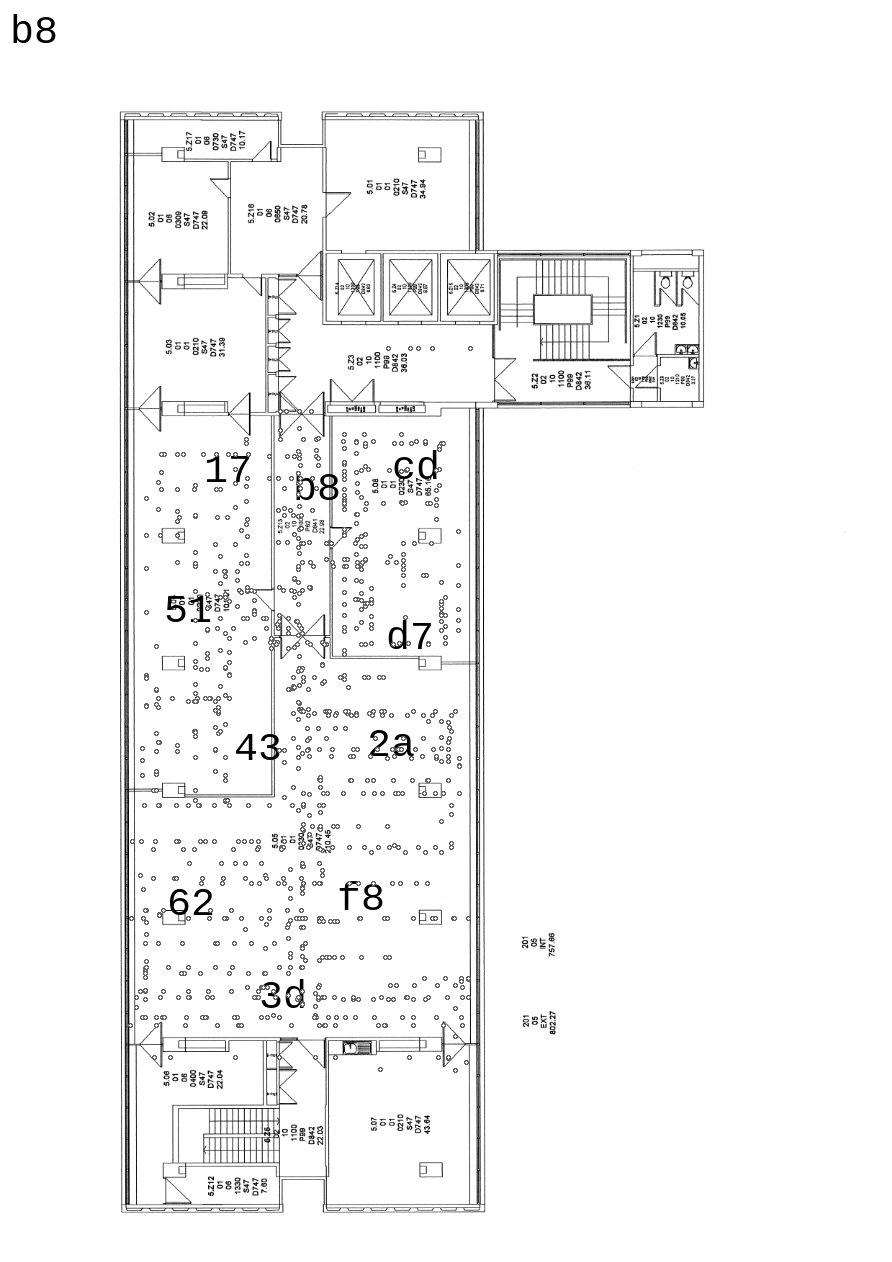
\includegraphics[width=\linewidth]{images/b8_read.png}
\column{0.5\textwidth}
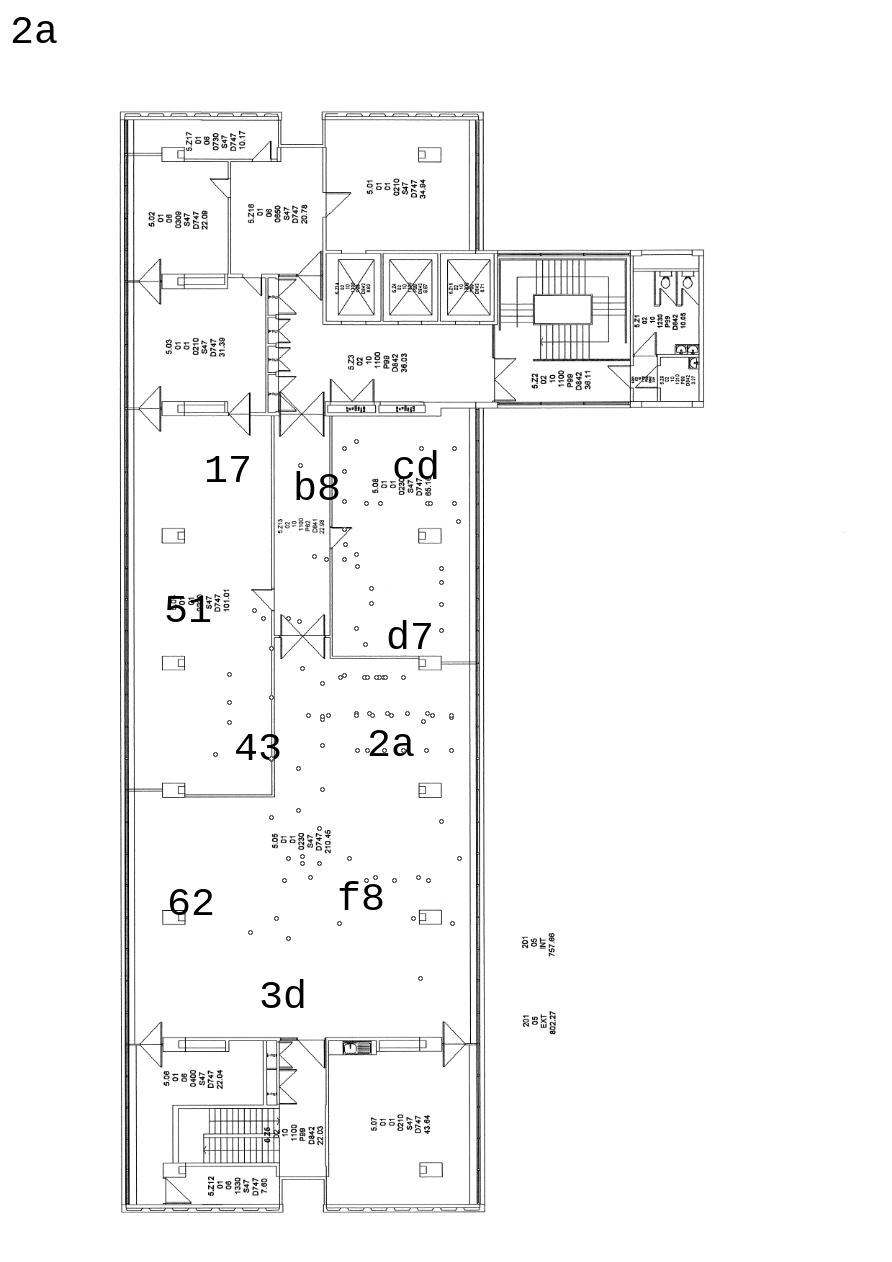
\includegraphics[width=\linewidth]{images/2a_read.png}
\end{columns}
\end{frame}

\begin{frame}
\frametitle{Conversion to/from global coordinates}
\begin{itemize}
\item We need to convert between global coordinates and pixel coordinates.
\item For the tiny area of a building, we can approximate spherical coordinates with Cartesian coordinates.
\item We translate the coordinates vectors so that the origin is at the NE corner of the floor, and then perform rotation and scaling by multiply a vector by a 2x2 matrix (or its inverse).
\item The conversion matrix was found by taking the global / pixel coordinates of three points and solving a linear equation.
\end{itemize}
\end{frame}

\begin{frame}
\frametitle{Does free-space propagation model hold?}
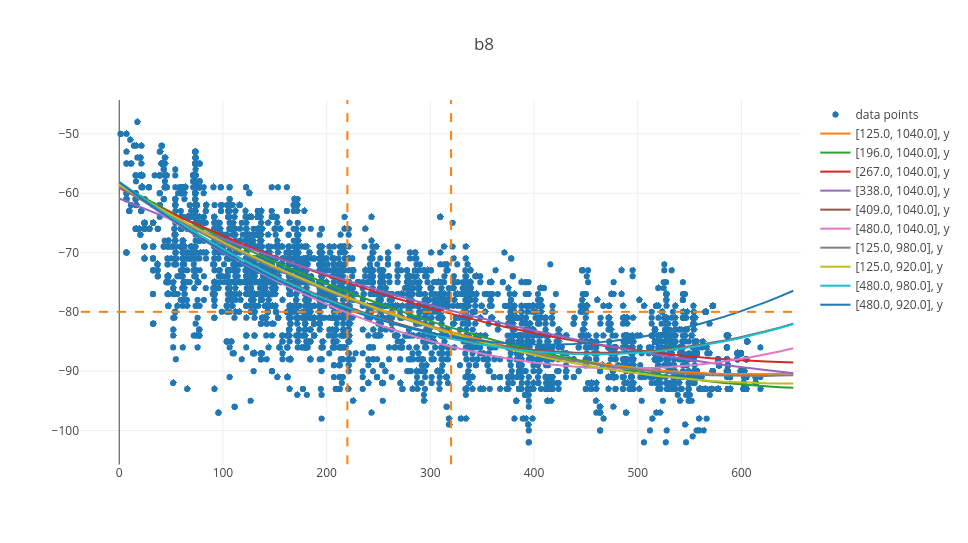
\includegraphics[width=\linewidth]{images/different_directions.png}
\end{frame}

\begin{frame}
\frametitle{Idea: trilateration on beacons 17 and b8}
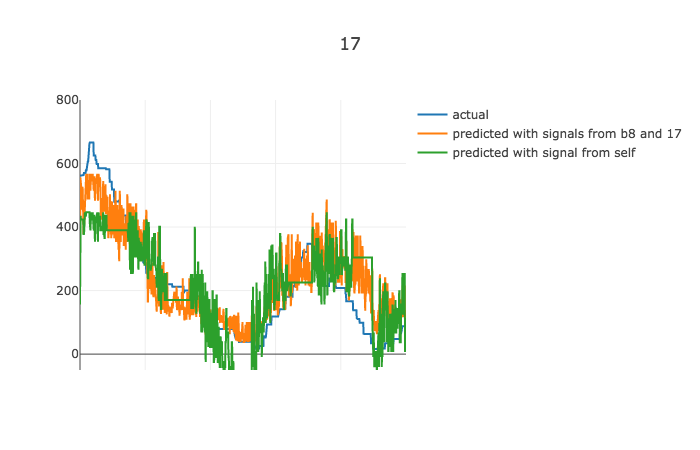
\includegraphics[width=\linewidth]{images/dist_f_rssi_17.png}
\end{frame}

\begin{frame}
\frametitle{Idea: trilateration on beacons 17 and b8}
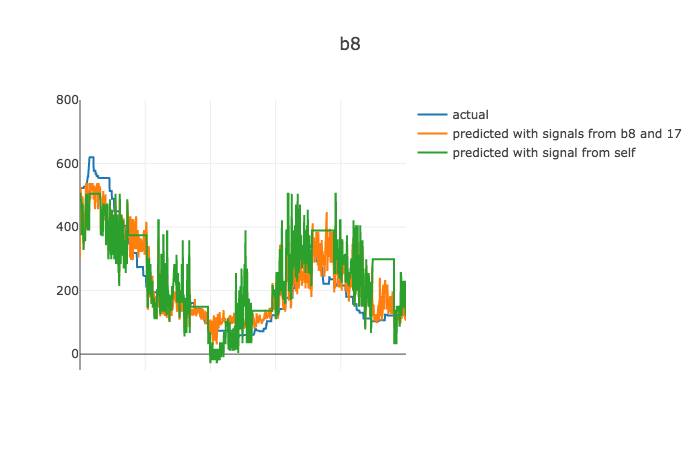
\includegraphics[width=\linewidth]{images/dist_f_rssi_b8.png}
\end{frame}

\end{document}





















